\documentclass[pdflatex,11pt]{aghdpl}
% \documentclass{aghdpl}               % przy kompilacji programem latex
% \documentclass[pdflatex,en]{aghdpl}  % praca w jezyku angielskim
\usepackage[polish]{babel}
\usepackage[latin2]{inputenc}
\usepackage{listings}
\usepackage{color}
\usepackage{listings}

% dodatkowe pakiety
\usepackage{enumerate}
\usepackage{listings}
\lstloadlanguages{TeX}

\definecolor{gray92}{gray}{.92}
\definecolor{gray75}{gray}{.75}
\definecolor{gray45}{gray}{.45}

\lstdefinestyle{source_code}
{
numbers=left,
stepnumber=5, 
basicstyle=\tiny, 
captionpos = b, %bottom 
keywordstyle=\color[rgb]{0,0,1}, 
commentstyle=\color[rgb]{0.133,0.545,0.133}, 
stringstyle=\color[rgb]{0.627,0.126,0.941}, 
backgroundcolor=\color{gray92}, 
frame=lrtb, 
framerule=0.5pt, 
linewidth = \textwidth 
}
 
\lstdefinestyle{console} 
{ 
numbers=none, 
basicstyle=\bf\ttfamily, 
backgroundcolor=\color{gray92}, 
frame= lrtb, 
framerule=0.5pt, 
linewidth=\textwidth, 
}

%---------------------------------------------------------------------------

\author{Pawe� Malczyk}
\shortauthor{Pawe� Malczyk}

\titlePL{Przygotowanie pracy dyplomowej w~systemie \LaTeX}
\titleEN{Thesis in \LaTeX}

\shorttitlePL{Przygotowanie pracy dyplomowej w~systemie \LaTeX} 
\shorttitleEN{Thesis in \LaTeX}

\thesistypePL{Praca magisterska}
\thesistypeEN{Master of Science Thesis}

\supervisorPL{dr Aleksander Byrski}
\supervisorEN{Aleksander Byrski Ph.D}

\date{2011}

\departmentPL{Katedra Automatyki}
\departmentEN{Department of Automatics}

\facultyPL{Wydzia� Elektrotechniki, Automatyki, Informatyki i Elektroniki}
\facultyEN{Faculty of Electrical Engineering, Automatics, Computer Science and Electronics}

\acknowledgements{Serdeczne dzieki itp.}



\setlength{\cftsecnumwidth}{10mm}

\begin{document}
\titlepages
\tableofcontents
\clearpage
\chapter{Wprowadzenie}
\label{cha:wprowadzenie}

Od pewnego czasu daje si� zaobserwowa� system�w opartych rozwi�zania typu
Workflow. Systemy te pozwalaj� na realizacj� pewnej logiki zwanej procesem w
okre�lony definiowalny spos�b. Do definiowania procesu stosuje si� struktury
grafowe opisuj�ce algorytm realizacji okre�lonego zadania. Opis grafu procesu
mo�e by� realizowany wieloraki spos�b jednak najcze�ciej s� to dokumenty XML o
semantyce opisuj�cej graf procesu. Obecnie najbardzie rozwijane jezyki definicji
opisu procesu to BPEL rozijany przez IBM, Microsof czy Bea Systems
(obecnie Oracle) czy XPDL rozwijany i standarywzowany przez organizacj�
workflow management coallition. W sk�ad WfMC wchodz� obecnie takie firmy jak
Fujitsu Computer Corporation, NEC Software limited, czy TIBCO Software, Inc.
W tym miejscu nasuwa si� pytanie czy rozwi�zania typu workflow mo�na by
wykorzysta� do zastosowa� naukowych, realizacji oblicze� zw�aszcza ewolucyjnych.
Ot� wi�kszo�� algorytm�w zw�aszcza oblicze� ewolucyjnych daje si� przedstawi� w
postaci grafu, a co za tym idzie, mo�na opisa� jak�� form� j�zyka definicji
proces�w oraz zaporzyczy� niekt�re koncepcje z klasycznych rozwi�za� workflow.
Przedstawienie obliczenia w postaci grafy daje mo�liwo�� �atwej zmiany
implementacji poszczeg�lnych frament�w obliczenia np. Metody krzy�owania, czy
selekcji bez konieczno�ci zmiany kodu. G��wnym celem pracy jest dostarczenie
rozwi�zania kt�re b�dzie da mo�liwo�c realizacji oblicze� przy u�yciu modelu
przedstawionego powy�ej. Platforma realizowana jako cze�� praktyczna b�dzie
zawiera� w sobie implementacja silnika, kt�ry maj�c opis realizacji obliczenie
przeprowadzie je odpoiedni spos�b. Interfejs programistyczny zawieraj��y zestaw
interfejs�w oraz adnotacji Javy. Jako cze�� projektu zaimplementowany zostanie
modu� zarz�dzaja�e wez�ami obliczenowymi i zlecaniem poszczeg�lnych zada�
obliczeniowych. Graficzny interfejs u�ytkownika zaimplementowany zostanie w
�rodowisku WWW i udost�pniny b�dzie za po�rednictwem protoko�u HTTP. Rozwi�zanie
to udost�pni dost�p do systemu ka�demu u�ytkownikowi kt�ryma sposobno�� u�ycia
przegl�drki internetowej niezale�nie od �rodowiska w jakim na codzie� pracuje.
Zastosowanie procesu oblicze� jako modelu ich realizacji sprzyja realizacji
koncepcji ponownego u�ycia poszczeg�lnych fragment�w kodu oblicze�. Poszczeg�lne
obliczenia b�d� wsp�dzielone pomi�dzy u�ytkownik�w. Takie podej�cie pozwoli
u�ytkownikom u�ycie zaimplementowanych ju� oblicze� jako cz�� ich w�asnego
procesu obliczeniowego. Istotna kwestia jest tak�e spos�b konfigurowalno��
prezentacji wynik�w oblicze� co umo�liwi potencjaln� integracj� z zewn�trznymi
systemami.

\section{U�yte Technologie}
\label{sec:technologie}
\begin{enumerate}
  \item Apache Ant (1.7.1) http://ant.apache.org/ Apache ANT - narz�dzie
  pocz�tkowo stworzone w celu automatyzacji proces�w budowania oprogramowania.
  Proces budowania opisany jest w dokumencie XML zawieraj�cym cele oraz
  zale�no�ci mi�dzy nimi. Narz�dzie ANT dostarczone jest z ca�ym pakietem
  wbudowanych implementacji zada� kt�re mog� by� u�yte do kompilacji, budowania
  wynikowej dystrybucji, testowania aplikacji oraz wielu innych typowych zada�
  realizowanych w procesie tworzenia oprogramowania. Narz�dzie to jest silnie
  rozszerzalne poprzez system wtyczek oraz oraz bibliotek. W projektcie poza
  typowymi zadaniami zwi�zanymi z kompilacj� i tworzeniem dystrybucji
  testowaniem aplikacji i tworzeniem dokumentacji, u�ywany jest tak�e to
  generowania schemat�w bazy danych oraz realizacji dalszych migracji,
  konfiguracji serwera aplikacji.
  \item Apache Tomcat (7.0) http://tomcat.apache.org/ Jeden z
  najpopularniejszych kontenerow aplikacji web zbudowanych z Servlet�w oraz
  Stron JSP. W tym projektcie jest zainstalowany na w�z�ach typu Slave i
  udostp�nia logik� obliczeniow� za po�rednictwem protoko�u Hessian\newline
  Pocz�tki Serwera Tomcat si�gaj� pocz�tk�w technologii Serwlet�w. W 1999 roku
  Sun Microsystems przekaza� kod kontenera serwlet�w Fundacji Apache,kt�ra
  wcze�niej ju� pracowa�a nad podobnym projektem o nazwie JServ. Z po��czenia
  obu produkt�w powasta�o oprogramownie kontenera serwerlet�w o nazwie Tomcat.
  Server Tomcat rozpowrzechniany jest na licencjach GPL oraz LGPL.( zr
  Proffesional apache tomcat 5)
  \item Apache Velocity (1.6.4) http://velocity.apache.org/ Silnik szablon�w
  pozwalaj�cy na wype�nianie zadanego szablonu odpowiednimi warto�ciami w miescu
  gdzie zdefinowana jest odpowiednia zmienna. W aplikacji szeroko stosowany to
  generowania tresci HTML wiadomo�ci email, a tak�e do tworzenia dokument�w
  XML kt�re zasilaj� danymi bibliotek� generuj�c� wykresy obci��e� serwer�w.
  Innymi typowymi zastosowaniami biblioteki mog� by� generatory kodu oraz strony
  html zawieraj�ce odpowiednie miejsca kt�re w momencie wy�wietlenia strony
  zostan� wype�nione dynamicznymi danymi.
  \item Apache Struts (2.1.8) http://struts.apache.org/ Apache Struts - Framwork
  realizuj�cy wzorzec MVC (Model-View-Controller) u�ywany do realizacji
  graficznego interfejsu u�ytkownika aplikacji. Struts dostarcza wygodne
  mechnizmy konfiguracji frameworka za pomoc� plik�w konfiguracyjnych XML, lub
  za pomocn� adnotaci Javy. Istotn� zalet� jest model programowania, oraz
  �atwo�� mapowania danych formularza na na odpowiadaj� im reprezentacj� w
  modelu. Tak�e i w tym frameworku istnieje mo�liwo�� do��czania wtyczek
  rozszerzaj�ych jego funkcjonalnosc w zale�no�ci od istniej�cych potrzeb.
  Przyk�adem mog� by� tutaj u�yte wtyczki kt�re umo�liwiaj� konwersj�
  zwracanych obiekt�w Javy do formatu JSON u�ywanego przez widok, b�d� wtyczka
  integruj�ca Struts z Velocity na potrzeby tworzenia wykres�w, b�d� Tiles. 
  \item Apache Tiles (2.0.6) http://tiles.apache.org/ Dostarcza dogodnych
  narz�dzi definiowania wygl�du graficznego interfejsu u�ytkownika. Framework
  pozawla na osi�gni�cie wysokiego stopnia ponownego u�ycia
  dowolnych fragment�w element�w grafcznego inerfejsu u�ytkownika. 
  \item Apache Digester (2.0) http://digester.apache.org/ Biblioteka u�ywana do
  zastosowa� realizuj�cych mapowanie dokument�w XML na obieky Javy. Istotn�
  zalet� jest szybko�� jego dzia�ania wynikaj�ca z faktu, �e mapowanie odbywa
  si� na bie��co w trakcie czytania dokumentu XML (nie ma potrzeby tworznia
  reprezentacji dokumentu w pamieci). Mapowanie w trakcie czytania jest sterowane zdarzeniowo, 
  a metoda mapowania konfigurwana jest przy pomocy okre�lonych regu�
  opisuj�cych wzore kt�re s� mapowane przez silnik na odpowiednie operacje
  realizowane na mapowanym obiekcie.
  \item Jakarta Cactus (1.8.1) http://jakarta.apache.org/cactus/ Jakarta Cactus
  - biblioteka umo�liwiaj�ce realizacj� test�w automatycznych komponent�w
  osadzonych na serwerze. W projekcie u�ywane do realizacji automatycznych
  test�w komponent�w EJB realizuj�cych w�a�ciw� logik� biznesow�.
  \item Java 1.6 http://www.oracle.com/technetwork/java/index.html jest
  obiektowym j�zykiem programowania og�lnego przeznaczenia. Kod wykonywane jest
  w obr�bie wirtualnej maszyny javy (JVM), tote� kod napisy w Java mo�e by�
  wykonywany w dowolnym �rodowisku na kt�ry zainstalowana jest maszyna.
  \item Liquibase (1.9.5) http://www.liquibase.org/ Liquibase - umo�liwia
  wygodne zarz�dzanie zmianami w modelu danych  w trakcie realizacji projektu.
  Biblioteka u�ywana do tworzenia schematu bazy danych, a nast�pnie wprowadzaniu
  przytostowych zmian w schemacie.
  \item PostgreSQL (9.0) http://www.postgresql.org/ PostgreSQL - szeroko stosowany,
  otwarto�r�d�owych system zarz�dzania relacyjnymi bazami danych. Pocz�tkowo
  rozwijany pocz�wszy od lat siedemdziesi�tych na Uniwersytecie kalifornijskim
  Berkeley. Silnik bazodanowy wspiera model realacyjny umo�liwia tworzenie
  widok�w nak�adania ogranicze� zapewniaj�cych integralno�� danych w tym
  wsparcie na stosowanie kluczy obcych. Silnik wspiera tworzenie procedur kt�re
  mog� by� zaimplementowane w j�zykach takich jak PL/Perl, plPHP, pl/Python,
  PL/Java. Kolejn� cech� jest mo�liwo�� stosowania indeks�w kt�re szybszy dost�p
  do potrzebnych danych. Mo�liwe typy indeks�w z kt�rych mo�na skorzysta�
  budowane s� w oparciu o B-Drzewo, R-Drzewo b�d� Hash. Silnik bazodanowy
  postgreSQL dostarcza twa podstawowe mechanizmy realizacji transakcyjno�ci. Sa
  nimi MVCC (MultiVersion Concurrency Control) oraz Two Phase Commit Protocol
  stosowany g��wny gdy mamy do czynienia z transakcjami obejmuj�cymi wi�ksza
  liczb� zasob�w transkacyjnych. Dodatkowymi istotnymi cechami tego silnika s�
  otwarta licencja (BSD) oraz mo�liwo�� kompilacji silnika na wiele r�znych
  typ�w platform.
  \item Quartz (1.7.1) http://www.quartz-scheduler.org/  Quartz - ma za zadanie
  cykliczne wyzwalane zdefiniowanych zada�. Pe�ni role podobn� do tej jak� pe�ni 
  CRON w systemach UNIX. Zalet� s� wysokie mo�liwo�ci konfiguracyjne.
  \item Glassfish Enterprise Server v.2.1.1 http://glassfish.java.net/ Glassfish
  Enterprise Server - Jest serwerem aplikacji, kt�ry implementuje interfejsy w
  ramach specifikacji JEE5. Do tych zaliczaj� si� kompnenty EJB(Enterprise Java
  Beans), oraz MDB(Message Driven Beans), JMS(Java Messaging Services) itp.
  Wen�trz serwera wbudowany jest tak�e kontener Tomcat, kt�ry udost�pnia
  graficzny interfejs u�ytkownika aplikacji.
  \item Hessian (4.0.7) http://hessian.caucho.com/ Hessian-Jest protoko�e,
  u�ywanym do zdalnego uruchamiania operacji. Istotn� zalet� jest to, �e nie jest ca�kowicie binarny jak RMI, 
  tylko bazuje na wymianie dokument�w XML. Wymieniane dokumenty, s�znacznie
  prostrze i kt�rsze ni� te z znane protoko�u SOAP.
  \item XStream (1.3.1) http://xstream.codehaus.org/ - Biblioteka u�ywana do
  serializacji i deserializacji zwracanych wynik�w oblicze� z wez��w slave.
  \item EJB (3.0) http://www.oracle.com/technetwork/java/index-jsp-140203.html EJB-Stosowane do realizacji logiki biznesowej aplikacji. 
  Zale�nie czy stanowe, czy nie mog� by� wymieniane pomi�dzy klientami, b�d�
  mog�  by� zaw�aszczone na czas trawania sesji. Zwykle realizowane w kontekscie
  transakcyjnym. W wersji 3 znacznie l�esze ni� te znane z wersji 2.x. Wygoda
  ich u�ycia sta�a si� g��wn� przyczyn� ich u�ycia.
  \item JPA(1.0) http://www.oracle.com/technetwork/articles/javaee/jpa-137156.html
  -Jest specyfikacja utrwalania obiekt�w w bazie danych za pomoc� mapowania obiektowo relacyjnego. Wygodna konfiguracja przy pomocy adnotacji Javy nie wymaga tworzenia dlugich dokument�w mapowa� jak to ma miejsce w
  przypadku Hibernate. JPA czesto jako silnika utrwalania u�ywa w�a�nie
  Hibernate.
  \item Amcharts http://www.amcharts.com/ Amcharts-U�ywane do generowania
  wszelakiego typu wykres�w. Narz�dzie dostarcza du�e mo�liwo�ci konfiguracji
  prezentowanych wykresu. Szeroki jest tak�e wachlarz dost�pnych typ�w wykres�w.
  Aby wygenerowa� wykres wystarczy zasili� bibliotek� dwoma dokumentami XML.
  PIerwszy ma za zadanie skonigurowanie wykresu pod k�tem jego typu oraz
  wygl�du, drugi ma za zadanie zasilic wykres danymi. Amcharts jakos dane
  akceptuj� zar�wno pliki XML jak i CSV.
  \item Jquery (1.4.1) http://jquery.com/ Biblioteka Java script og�lnego
  przeznaczenia. Jquery dostarcza wygodne techniki manipulowania drzewem DOM
  wy�wietlanej strony poprzez zestaw wbudowanych selektor�w. Dodatkowo dostarcza
  mo�liwo�� �atwego tworzenia ��da� ajax i obs�ugi zwracanych danych. Istotn�
  spraw� jest tak�e to i� jego architektura jest rozszerzalna poprzez mechanizm
  wtyczek. 
  \item Jqgrid - Jest wtyczk� do frameworka Jquery kt�ra umo�liwa �atwe
  tworzenie tabel, stronicowania sortowanie itp. Tabele zasilane s� poprzez dane
  w formacie JSON.
  \item Apache FOP - http://xmlgraphics.apache.org/fop/ Implementacja standardu
  XSL-FO u�ywany do generowania plik�w PDF z dokument�w XML.
  \item Checkstyle - Jest narz�dziem deweloperskim, kt�re pozawala na
  degfinowanie regu�, kt�re musz� by� przestrzegane w trakcie tworzenia
  oprogramowania. Sprawadzanie kodu pod k�tem zdefiniowanych uprzednio regu�
  odbywa si� w trakcie budowania dystrybucji oprogramowania. Dodatkowo narz�dzie
  to posiada zestaw wtyczek do popularnych �rodowisk programistycznych takich
  jak eclipse b�d� netbeans. 
  \item PMD - pe�ni zbli�on� funkcj� do tej tej realizowanej przez checkstyle.
  Dodatkowo u�atwia analizuje kod pod k�tem mo�liwych b��d�w na podstawie
  pustych block�w try/catch/finally, zduplikowanego i ma�o optymalnego kodu a
  tak�e zbyt skomplikowanych mo�liwych scie�ek realizacji programu. 
  \item JSch - Biblioteka implementuj�ca operacje protoko�u SSH/SFTP. Za jej
  pomoc� zaimplementowane jest rozsy�anie konfiguracji oraz pakiet�w oblicze�
  na serwery Slave przy u�yciu protoko�u SFTP.
  \item Servlety, JSP (Java Server Pages) - Obie technologie s�u�� do
  realizacji dynamicznych stron WWW. Serwlety dostarczaj� pewn� porcj� logiki,
  kt�ra w dynamiczny spos�b tworzy pewn� dynamiczn� tre��. 
  Pomimo faktu, �e specyfikacja serwlet�w nie ogranicza ich u�ycia przy zastosowaniu protoko�u
  HTTP, to zdecydowana wi�kszo�� tworzonych serwelet�w zawsze obs�uguje ��dania
  protoko�u HTTP jak GET/POST/PUT/DELETE. Strony JSP na osadzanie pewnej
  dynamicznej zawarto�ci w zwyk�ych statycznych stronach HTML. Strona JSP jest
  kompilowana przez kontener do postaci serwletu w momencie pierwszego wywo�ania
  takiej strony. Specyfikacja JSP pozwala na stosowanie tzw. bibliotek Tag�w
  kt�re dostarczaj� pewn� reu�ywalna logik� udost�pnian� za po�rednictwem
  odpowiednich tag�w.
\end{enumerate}

\chapter{Architektura}
Obliczenia wykonywane s� na w schemacie Master-Slave. Serwer master
odpowiedzialny jest za przygotownie obliczenia, do realizacji na
w�z�ach slave, koordynacji wykonania procesu obliczenia, logowanie zdarze�
zachodz�cych w trakcie realizacji obliczenia. Po zako�czeniu obliczenia 
dokonuje zapisu wynik�w oblicze� w bazie danych a nast�pnie wysy�any zostaje
email powiadamiaj�cy z zako�czeniu obliczenia wraz z linkiem do miejsca gdzie te
wyniki s� osi�galne.

Platforma obliczeniowa sk�ada si� z g��wnego serwera master, osadzonego na
serwerze Glassfish i zrealizowany w specyfikacji Java EE w wersji 5.
Na specyfikacje JEE sk�ada si� wiele interfejs�w programowania takch jak EJB,
JPA, JMS, JNDI i wiele innych. Cz�c z tych interfejs�w tworzenia
oprogramownia u�yta to realizacji aplikacji. Jedna z technologii kt�ra zosta�a
u�yta jest technologia EJB. Komponenety stworzone za po�rednictwem tej
technologi maj� za zadanie realizacj� w�a�ciwej logiki biznesowej aplikacji.
Specyfikacja przewiduje tworzenie dw�ch typ�w kompoenent�w stanowych, oraz
bezstanowych. Bezstanowe kompoenenty mog� by� wymieniane pomi�dzy wieloma
aplikacjami klienckimi, natomiast komponenety stanowe s� dowi�zane do
konkretnego klienta do czasu zako�czenia realizacji okre�onej logiki. Niemal
wsztkie funkcjonalno�ci platformy obliczeniowej zrealizowane s� za pomoc�
bezstanowych kompoenent�w EJB. Drugi z istotniejszych interfejs�w programownia
jest JPA. Specyfikacja ta opisuje metody otrwalania obiekt�w Javy w trwa�ym
repozytorium np. relacyjnej bazie danych. Ponadto dostarczony jest j�zyk do
realizacji zapyta�, oraz zestaw adnotaji Javy do opisu relacji pomi�dzy
utrwalanymi obiektami. Aplikacja rob u�ytek z dodatkowej warstwy
mapowania obiektowo relacyjnego (ORM)jak� w prowadza JPA do utrwalania wszelkich
potrzebnych obiekt�w. Funkcjonalno�ci kt�re z ich natury musz� by� realizowane w
spos�b asynchroniczny realizaowane s� za po�rednictwem wymiany komunikat�w i
specyfikacji JMS (cos wiecej?).

Wszystkie wez�y obliceniowe Slave posiadaj� zainstalowany serwer apache tomcat,
oraz prost� bezstanow� aplikacj� kt�ra dostarcza kliku prostych funkcjonalno�ci. 
Pierwsza  nich jest udost�pnianie informacji o bie�acych parametrach wirtualnej
maszyny na kt�rej jest uruchomiona. Kolejne funkcjonalno�ci dostarczane przez
aplikacj� dotycz� realizacji oblice� tj. przyjmowania �ada� realizacji
obliczenia, dynamicznego wyszukiwania i wczytywania klas oblicze�, w�a�ciwej
realizacji obliczenia oraz zwracania wynik� do serwera master.


  

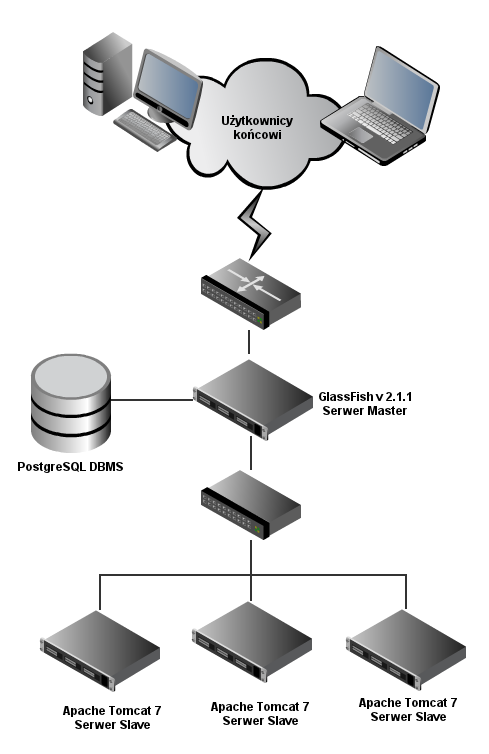
\includegraphics[scale=0.7]{gfx/MainView.png}

\section{Podzia� Projekt�w}
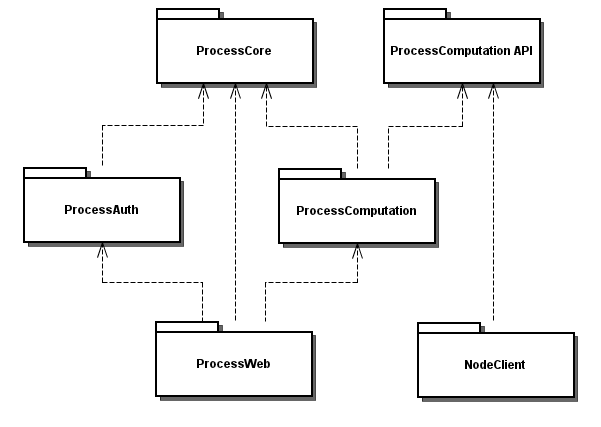
\includegraphics[scale=0.7]{gfx/packages.png}
\begin{enumerate}
  \item NodeClient - Zewn�trzna aplikacja dzia�aj�ca na serwerch slave
  udost�pniaj�ca za po�rednictwem protoko�u HTTP poszczeg�lne obliczenia.
  Odpowiedzialna jest za �adowanie potrzebnych bibliotek na rz�dzanie wykonanie
  obliczenia oraz serializacj� wynik�w. Drug� funkcjonalno�ci� jest
  udost�pnianie informacji o aktualnych parametrach wirtualnej maszyny Javy za
  po�rednictwem ava Management Extensions (JMX).
  \item ProcessCore - dostarcza nast�puj�ce funkcjonalno�ci
  	\subitem Obs�uga plik�w konfiguracyjnych aplikacji
  	\subitem Obs�uga parametr�w konfiguracynych aplikacji
  	\subitem Obs�uga plik�w
  	\subitem Ob�suga plik�w JAR przeszukiwanie zawarto�ci wydobywanie
  	konfiguracji.
  	\subitem Zdalne wywo�ywanie zada� na serwerach slave
  	\subitem Obs�uga cyklicznie powtarzalnych zada�
  	\subitem Generowanie plik�w PDF
  	\subitem Obs�uga szablon�w za po�rednictwem Veolcity
  	\subitem Obs�uga transformacji XSLT
  \item ProcessAuth dostarcza us�ugi zwi�zane z zarz�dzaniem grupami
  u�ytkownikow, oraz pojedynczymi u�ytkownikami. Zarz�dza histori� logowa�
  u�ytkownik�w, oraz ich uprawnieniami. \newline
  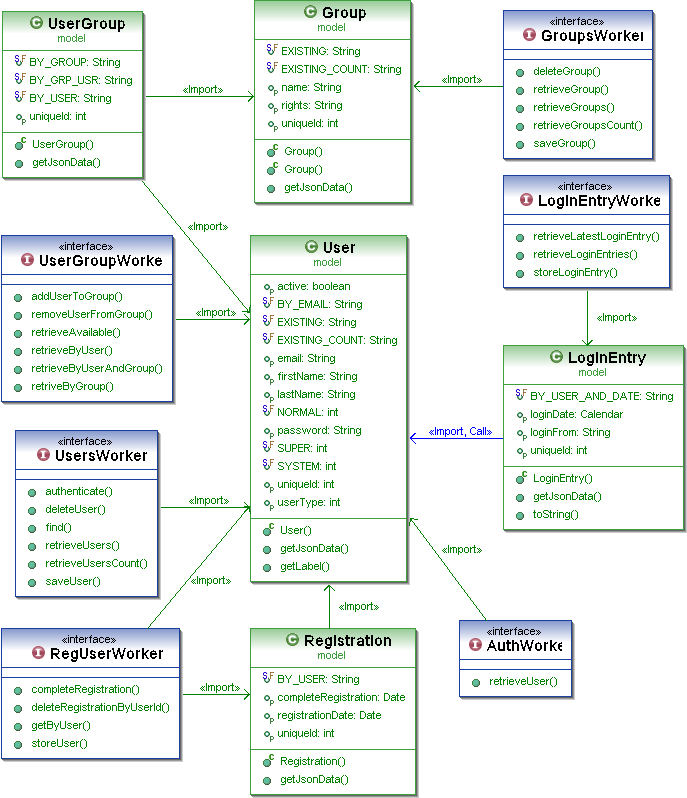
\includegraphics[scale=0.5]{gfx/auth.png}
  \item ProcessComputationApi - Dostarcze wszystkie s�adowe w postaci
  interfejs�w, adnotacji Javy koniecznych do tworzenia aplikacji obliczeniowych
  daj�cych si� uruchomi� na platformie.
  \item PrecessComputation - Enkapsuluje ca�kowit� logik� tworzenia oblicze� z
  pakiet�w oblicze� jak i konfiguracji. Ponadto w projekcie tym zawarta jest
  logika silnika realizuj�cego obliczenie wedle okre�lonej konfiguracji. 
  \item ProcessWeb - Stanowi warst� prezentacji projektu. Dostarcze graficzny
  interfejs u�ytkownika u�ytkownika.
\end{enumerate}
\section{Monitorowanie w�z��w slave}
Monitorowanie w�z��w odbywa si� za po�rednictwem technologi JMX (Java Management
Extensions). Aby mo�liwe by�o monitorowanie konieczne jest odpowiednie
skoniguraowanie zar�wno w�z��w slave oraz serwera master. Ka�dy z serwer�w
slave powienien mie� udost�pnione us�ugi JMX (wpisac gdzie to jest napisane), a
ponadto serwer Master powinienmiec zdefiniowane (napisane dalej co).
Monitorowanie w�z�a odbywa sie si� w nast�puj�cych krokach
\begin{itemize}
  \item Ka�dy z serwer�w wysy�a �adanie rejestruj�ce go w puli dost�pnych
  serwer�w slave, po tym jak zostaje zarejestrowany co pewien czas od�wierza
  swoja rejestracj�.
  \item Serwer master ma zaimplementowane zadanie zgodne z wytycznymi biblioteki
  Quartz, kt�re to ma za zadanie pobieranie informacji o aktualnych parametrach
  wirtualnej maszyny Javy na serwerach slave. Czestotliwo�� wyknania adania jest
  konfigurowalna przy pomocy odpowiedniego wyra�enia zblio�one syntaktyk� to
  tych stosowanych w narz�dziu CRON.
  \item Ka�da zebrana informacja na temat aktualnego obci��enia serwera jest
  zapisywana bazie danych. Na podstawie zebranych historycznych danych mo�liwa
  jest wizualzacja obicia�enie poszczeg�lnych w�z��w za po�rednictwem
  graficznego interfejsu u�ytkownika.
\end{itemize}
\subsection{Monitorowane parametry}
Specyfikacja JMX udost�pnia nazwane obiekty kt�rych atrybuty mo�na
odczytywa�/zmienia�. W przypadku projektu wykorzystane zosta�y trzy z nich:
\begin{itemize}
  \item java.lang:type=Runtime - za po�rednictwem tego obiektu pobierane sa
  informacje typie i dostawcy wirtualnej maszyny Javy.
  \item java.lang:type=Threading - za po�rednictwem tego obiektu pobierane sa
  informacje  ilo�� aktwnych w�tk�w.
  \item java.lang:type=OperatingSystem - atrybuty jakie s� osi�galne poprzez ten
  obiekt dostarczaj� informacji o typie systemu operacyjnego, architekturze
  systemu, ilo�� dost�pnych procesor�w, ilo�� pamieci fizycznej/wolnej,
  obci��enie procesor�w itp\ldots
\end{itemize}
\newpage

\subsection{Model danych}
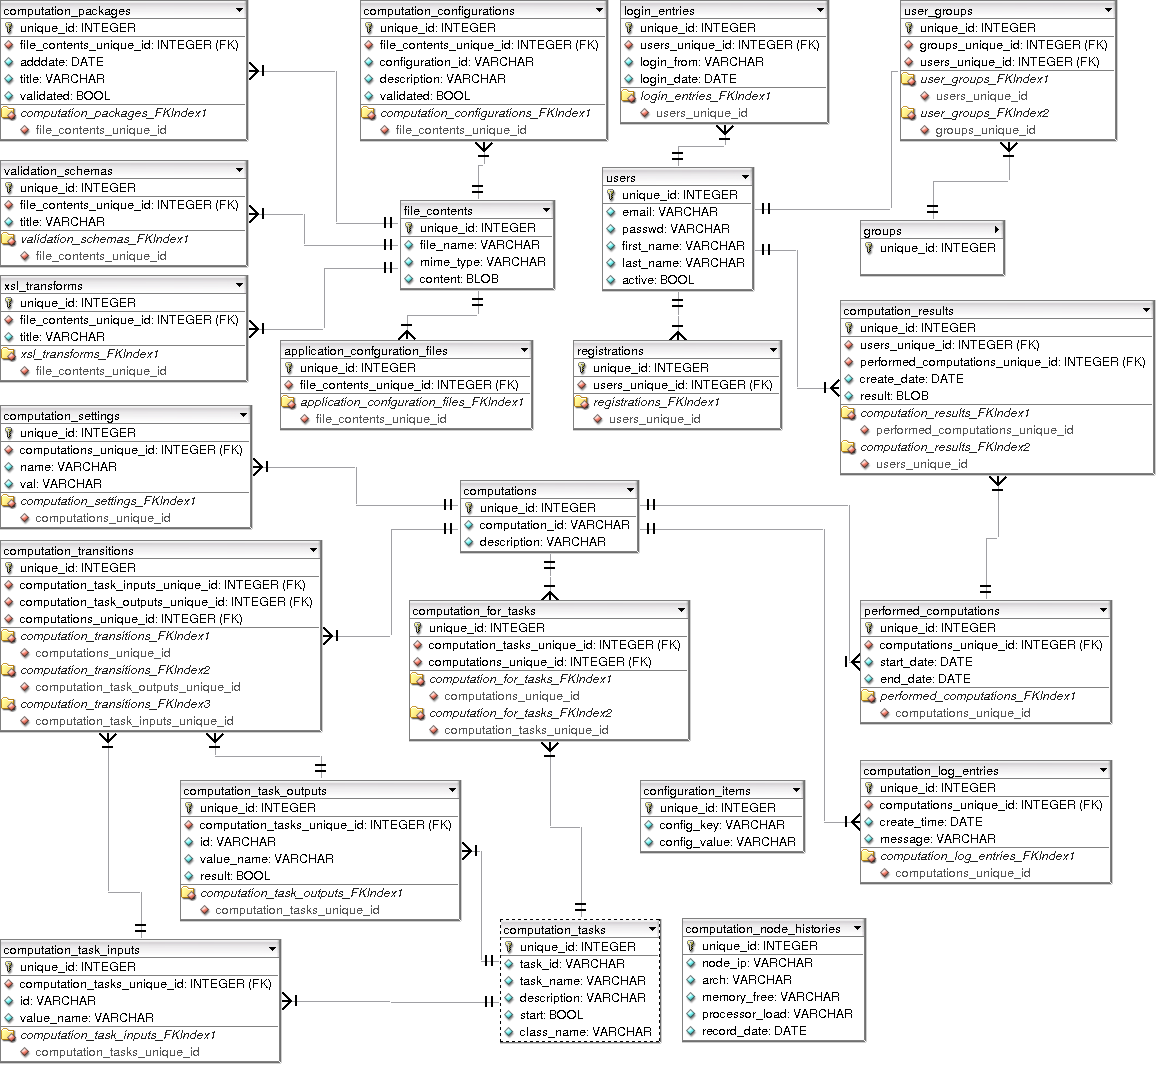
\includegraphics[scale=0.4]{gfx/db_model.png}
\newline
\begin{itemize}
  \item computation\_packages - dodanie pakietu obliczenie powoduje stworzenie
  odpowienieg wpisu w tej tabeli. Pole title zawiera czytelny dla cz�owieka
  tytu� obliczenia, kt�ry b�dzie wy�wietlany na elementach graficznego
  interfejsu u�ytkownika. W�a�ciwa zawarto�� pliku pakietu oblicze� przchowywana
  jest w tabeli file\_contents.
  \item validation\_schemas - przechowuje informacje o zaimportowanych plikach
  walidacyjnych.
  \item xsl\_transforms - pliki transformat XSLT kt�re zosta�y zaimporotwane do
  systemu posiadaj� odpowiedni wpis w tej tabeli. Podobnie jak w przypadku
  innych plik�w tak�e i zawarto�� tych jest przechowywana w tabeli
  file\_contents.
  \item computation\_settings - przechowuje ustawienia specyficzne dla
  poszczeg�lnego procesu obliczenia (zawarte w pomi�dzy elementami settings
  pliku konfiguracyjnego).
  \item computation\_transitions - przechwuje informacje o wszystkich
  przej�ciach pomi�dzy sk�adowymi obliczeniami.
  \item computation\_task\_inputs - przechwouje informacje o wej�ciach
  poszczeg�lnych dzia�a� o ich identifikatorze oraz zmiennej wej�ciowej
  obliczenia kt�r� reprezentuja.
  \item computation\_task\_outputs - przchowuje informacje o wyj�ciach
  obliczenia oraz zmiennej kt�rej warto�� b�dzie znajowa�a si� na wyj�ciu. 
  \item computation\_tasks - tu znajduj� si� wszystkie pojedyncze zadania
  obliczeniowe kt�re stanowi�ce reu�ywalna cz��, z kt�rych mo�na komponowa�
  procesy oblicze�.
  \item computation\_for\_Tasks - tabela ��cznikowa ��cz�ca pojedyncze zadanie
  obliczeniowe z procesem obliczeniowym.
  \item computations - zawiera wszystkie utworzone reprezentacje oblicze�
  bazuj�c na zaimortowanych pakietach oblicze� b�d� konfiguracji oblicze�.
  \item application\_configuration\_files - 
  \item file\_contents - Przechowuje wszystkie binarne pliki kt�re zosta�y
  za�adowane do platformy oblicze�.
  \item computation\_configurations przechowuje oddzielenie zaimportowane
  konfiguracje oblicze� w formacie XML. Tak�e i tu zawarto�� pliku ma swoje
  miejsce w tabeli file\_contents.
  \item login\_entries Wszystkie zdarzenia logowanie u�ytkownik�w s�
  rejestrowane w tej tabeli.
  \item users tabela u�ytkownik�w.
  \item user\_groups tabela ��cznikowa ��cz�ca u�ytkownik�w z grupami.
  \item groups lista group u�ytkownik�w
  \item registrations- zawiera informacje o przeprowadzonej rejstracji
  u�ytkownika. Na podastawie wpis�w tej tabeli dokonywana jest aktywacja konta.
  \item configuration\_items - przechowuje zmienne i warto�ci kofiuguracyjne dla
  ca�ej aplikacji.
  \item computation\_node\_histories zawiera wpisy z odczytami parametr�w
  zdalnych wirtualnych maszyn JAVy na serwerach slave.
  \item computation\_log\_entries - poszczeg�lne zdarzenia zwi�zane z realizacj�
  procesu obliczeniowego s� rejestrowane i wpisy tego typu znajduj� si� w tej
  tabeli.
  \item performed\_computations  wszyskie historycznie wykonane obliczenia maj�
  odpowiedni wpis w tej tabeli.
  \item computation\_results  po uprzednim wykonaniu obliczenia wyniki oblicze�
  s� przechowywane w tej tabeli.
\end{itemize}

\chapter{Konfiguracja i budowanie aplikacji}
Do automatyzacji procesu budowania u�yte zosta�o narz�dzie Apache ANT. Dzi�ki
temu wi�kszo�� czynno�ci zwi�zanych z budowaniem oraz konfigurowaniem aplikacji
sprowadza si� do uruchomienia konkretnego celu narz�dzia ANT.  
Aby mo�liwe by�o poprana konfiguracja parametr�w aplikacji konieczne jest
ustawienie zmiennej TASK\_HOME wskazuj�cej na katalog w kt�rym znajduje si�
plik config.properties zawieraj�cy zmienne konfiguracyjne wraz z odpowiednimi
warto�ciami.

\section{Zmienne konfiguracyjne}
Zmienne serwera bazodanowego:
{\tiny
\begin{lstlisting}[style=console, caption=A command] 
db.jdbc.driverClassName=klasa sterownika JDBC
db.jdbc.url=URL po�aczenia JDBC uwzgl�dniaj�ca nazw� bazy danych aplikacji
db.jdbc.url.pg=URL po�aczenia JDBC u�ywa przy tworzeniu bazy danych
db.jdbc.username=login u�ytkownika u�yte przy po��czeniu z u�yciem JDBC
db.jdbc.password=has�o u�ytkownika u�yte przy po��czeniu z u�yciem JDBC
db.changelog.file=changelog.xml nazwa pliku wskazuj�ca na migracje danych
db.name=nazwa bazy danych
\end{lstlisting}
} 


Zmienne serwera master (Glassfish):
{\tiny
\begin{lstlisting}[style=console, caption=A command] 
glassfish.lib=katalog zawieraj�cy biblioteki serwera
glassfish.home=katalog g��wny serwera glassfish
glassfish.admin.username=login u�ytkownika administracyjnego 
glassfish.admin.passwd=has�o u�ytkownika administracyjnego
glassfish.admin.passwdfile=lokacja pliku z has�em do cel�w administracyjnych 
glassfish.domain.name=nazwa domeny administracyjnej
\end{lstlisting}
}
Zmienne serwera slave (Tomcat)
{\tiny
\begin{lstlisting}[style=console, caption=A command] 
nodeClient.app.path=scie�ka kontekstowa aplikacji
nodeClient.tomcat.manager.user=login u�ytkownika administracyjnego serwera
nodeClient.tomcat.manager.password=has�o u�ytkownika administracyjnego serwera
nodeClient.tomcat.url=URL panelu administracyjnego serwera
nodeClient.root=G��wny katalog projektu
nodeClient.dist=katalog zawieraj�cy dystrybucj� projektu
\end{lstlisting}
}
Zmienne serwera pocztowego
{\tiny
\begin{lstlisting}[style=console, caption=A command] 
mail.from=pole from wiadomo�ci email
mail.smtp.user=u�ytkownik serwera SMTP
mail.smtp.host=adres serwera SMTP
mail.smtp.port=port serwera SMTP
mail.smtp.password=has�o serwera SMTP
\end{lstlisting}
}
Zmienne konfiguracyjne projekt�w
{\tiny
\begin{lstlisting}[style=console, caption=A command] 
application.url=http://localhost:8080/procc
core.name=ProcessCore
core.root=/home/malczyk/Devel/Java/taskworkflow/ProcessCore
core.dist=/home/malczyk/Devel/Java/taskworkflow/ProcessCore/dist
core.build=/home/malczyk/Devel/Java/taskworkflow/ProcessCore/build
core.tests=/home/malczyk/Devel/Java/taskworkflow/ProcessCore/buildtest
common.lib=/home/malczyk/Devel/Java/taskworkflow/ProcessCore/lib
computationApi.root=/home/malczyk/Devel/Java/taskworkflow/ProcessComputationApi
computationApi.dist=/home/malczyk/Devel/Java/taskworkflow/ProcessComputationApi/dist
computation.root=/home/malczyk/Devel/Java/taskworkflow/ProcessComputation
computation.dist=/home/malczyk/Devel/Java/taskworkflow/ProcessComputation/dist
computation.build=/home/malczyk/Devel/Java/taskworkflow/ProcessComputation/build
computation.tests=/home/malczyk/Devel/Java/taskworkflow/ProcessComputation/buildtest
auth.root=/home/malczyk/Devel/Java/taskworkflow/ProcessAuth
auth.dist=/home/malczyk/Devel/Java/taskworkflow/ProcessAuth/dist
auth.build=/home/malczyk/Devel/Java/taskworkflow/ProcessAuth/build
auth.tests=/home/malczyk/Devel/Java/taskworkflow/ProcessAuth/buildtest
test.data=/home/malczyk/Devel/Java/taskworkflow/TestData
\end{lstlisting}
}

\section{Konfiguracja Aplikacji}
\subsection{Konfiguracja Serwera Bazodanowego}
Do inicjalizacji bazy danych oraz wykoanania wszystkich przyrostowych skrypt�w
SQL odpowiedzialnych za stworzenie schematu oraz wykonanie wszystkich migracji
odpowiedzialne s� kolejne cele ANT'a.
Ich uruchomienie mo�liwe jest z katalogu ProcessWeb

\subsubsection{Tworzenie bazy danych.}
{\tiny
\begin{lstlisting}[style=console, caption=A command] 
malczyk@linux-ln5n:~/Devel/Java/taskworkflow/ProcessWeb> ant create-database
Buildfile: build.xml

create-database:
      [sql] Executing commands
      [sql] 1 of 1 SQL statements executed successfully

BUILD SUCCESSFUL
Total time: 1 second
\end{lstlisting}
}

\subsubsection{Tworzenie schematu i wykonanie przyrostowych migracji danych}
Tutaj process uaktualniany jest przez narz�dzie LiquiBase gwarantuj�ce wykonanie
wszystkich przyrostowych skrypt�w SQL, stworzonych we wszystkich
zale�nych projektach.

{\tiny
\begin{lstlisting}[style=console, caption=A command] 
malczyk@linux-ln5n:~/Devel/Java/taskworkflow/ProcessWeb> ant update-database
Buildfile: build.xml

update-database:

prepare-liquibase:

update-database:
[updateDatabase] Create Database Lock Table
[updateDatabase] Lock Database
[updateDatabase] Successfully acquired change log lock
[updateDatabase] Create Database Change Log Table
[updateDatabase] Creating database history table with name: databasechangelog
[updateDatabase] Reading from databasechangelog
[updateDatabase] Changeset classpath:/changelog.xml::core_1::Pawel Malczyk::(MD5Sum: 9134232fa6ec6c9ad6d7e2b3e4ece34)
[updateDatabase] Changeset classpath:/changelog.xml::core_2::Pawel Malczyk::(MD5Sum: 7f18e87081b4d4b5329eec9c83d5e91)
[updateDatabase] Changeset classpath:/changelog.xml::core_3::Pawel Malczyk::(MD5Sum: 92bdd1cf3ea7aee4427bb85594c4196f)
[updateDatabase] Changeset classpath:/changelog.xml::core_4::Pawel Malczyk::(MD5Sum: cda3759dabcd714a43ff6f85595984a4)
[updateDatabase] Changeset classpath:/changelog.xml::core_5::Pawel Malczyk::(MD5Sum: 6c85c17c5c7a8bc8c3d792c0d780ded7)
[updateDatabase] Release Database Lock
[updateDatabase] Successfully released change log lock

.................................................................................................

BUILD SUCCESSFUL
Total time: 7 seconds

\end{lstlisting}
}

\subsubsection{Usuwanie bazy danych.}

{\tiny
\begin{lstlisting}[style=console, caption=A command] 
malczyk@linux-ln5n:~/Devel/Java/taskworkflow/ProcessWeb> ant drop-database
Buildfile: build.xml

drop-database:
      [sql] Executing commands
      [sql] 1 of 1 SQL statements executed successfully

BUILD SUCCESSFUL
Total time: 1 second
\end{lstlisting}
}




\subsection{Konfiguracja Serwera Master}
\subsubsection{Tworzenie domeny administracyjnej serwera glassfish}
Domena administracyjne serwera Glassfish definiuje skonfigurowane
izolowane �rodowisko umo�liwiaj�ce uruchamianie aplikacji. Dost�p do panelu
administracyjnego dost�pny jest za po�rednictwem protoko�u HTTP poprzez port
4848 i ile ten port nie zosta� jawnie wyspecyfikowany w momenci tworzenia domeny
administracyjnej. Ka�da domena administracyjna posiada w�asn� konfiguracj�,
pliki dziennik�w. Zmiany wprowadzone w obr�bie jednej z domen nie maj� wp�ywu na
dzia��nie aplikacji osadzonych w obr�bie innych domen administracyjnych.

{\tiny
\begin{lstlisting}[style=console, caption=A command] 
malczyk@linux-ln5n:~/Devel/Java/taskworkflow/ProcessWeb> ant create-domain
Buildfile: build.xml

create-domain:
     [exec] Using port 4848 for Admin.
     [exec] Using default port 8080 for HTTP Instance.
     [exec] Using default port 7676 for JMS.
     [exec] Using default port 3700 for IIOP.
     [exec] Using default port 8181 for HTTP_SSL.
     [exec] Using default port 3820 for IIOP_SSL.
     [exec] Using default port 3920 for IIOP_MUTUALAUTH.
     [exec] Using default port 8686 for JMX_ADMIN.
     [exec] Domain being created with profile:developer, as specified by variable AS_ADMIN_PROFILE in configuration file.
     [exec] ------ Using Profile [developer] to create the domain ------
     [exec] XML processing for profile: Base document 
     [/home/malczyk/Devel/tools/glassfish/lib/install/templates/default-domain.xml.template].
     Profile name [developer].\\ Processing property [domain.xml.style-sheets].
     [exec] [exec] The file in given locale [pl_PL] at:
     \\[/home/malczyk/Devel/tools/glassfish/lib/install/templates/locales/pl_PL/index.html]
     could not be found. Using default (en_US) index.html instead.
     [exec]Security Store uses: JKS [exec] Domain testdomain created.

BUILD SUCCESSFUL
Total time: 23 seconds

\end{lstlisting}
}
\subsubsection{Usuwanie domeny administracyjnej serwera glassfish}
{\tiny
\begin{lstlisting}[style=console, caption=A command] 
malczyk@linux-ln5n:~/Devel/Java/taskworkflow/ProcessWeb> ant drop-domain
Buildfile: build.xml

drop-domain:
     [exec] Domain testdomain deleted.

BUILD SUCCESSFUL
Total time: 1 second
\end{lstlisting}
}
\subsubsection{Tworzenie puli po��cze� JDBC}

Pula po��cze� JDBC jest przetrzymuje pewn� ilo�� po��cze� bazodanowych. 
Ustanowienie po��czenia z serwerem bazodanowym jest
czasoch�onne tote� pula po�acze� zarz�dzane przez siebie po��czenia podtrzymuje.
W momencie gdy aplikacja kliencka zarz�da dost�pu do serwera bazodanowego, pula
po��cze� udost�pni jedno z zarz�dzanych przez siebie po��cze�. Po zako�czeniu
dza�ania aplikacji klienckiej po��czenie zwracane jest do puli,
samo po��czenie pozostaje aktywne.

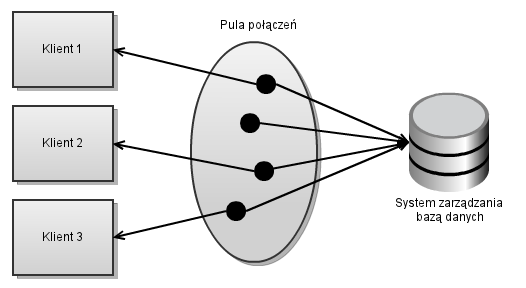
\includegraphics[scale=0.5]{gfx/pool.png}

{\tiny
\begin{lstlisting}[style=console, caption=A command] 
malczyk@linux-ln5n:~/Devel/Java/taskworkflow/ProcessWeb> ant create-jdbc-pool
Buildfile: build.xml

create-jdbc-pool:
     [exec] Command create-jdbc-connection-pool executed successfully.

BUILD SUCCESSFUL
\end{lstlisting}
}

W zale�no�ci od potrzeb istnieje mo�liwo�� dodatowej zmiany parametr�w puli
po��czen.
\begin{itemize}
  \item Initial and Minimum Pool Size - Okre�la startow� ilo�� po��cze�
  jaka b�dzie zarz�dzana przez pul�.
  \item Maximum Pool Size - Okre�la maksymaln� ilo�� po��cze� jak� pula mo�e
  obs�ugiwa�.
  \item Pool Resize Quantity - Warto�� ta okre�la ile nowych po��cze� do serwera
  bazodanowego zostanie ustanowionych w momencie kiedy wszystkie obecnie
  zarz�dzane po��czenia s� zaj�te i nadal istnieje mo�liwo�� ustanowienia nowych
  tj ilo�� zarz�dzanych po��cze� jest mniejsza niz przewiduje parametr Maximum
  Pool Size.
  \item Idle Timeout - Maskymalny czas braku aktywno�ci po kt�rym po��czenie
  zostanie zwr�cone do puli.
  \item Max Wait Time - Maksymalny czas jaki aplikacja kliencka b�dzie oczekiwa�
  na udost�pnienie po�aczenia z puli.
\end{itemize}

\subsubsection{Usuwanie puli po��cze� JDBC}
{\tiny
\begin{lstlisting}[style=console, caption=A command] 
malczyk@linux-ln5n:~/Devel/Java/taskworkflow/ProcessWeb> ant drop-jdbc-pool
Buildfile: build.xml

drop-jdbc-pool:
     [exec] Command delete-jdbc-connection-pool executed successfully.

BUILD SUCCESSFUL
Total time: 1 second
\end{lstlisting}
}
\subsubsection{Tworzenie zasobu JDBC w JNDI}

JNDI (Java Naming and Directory Interface) dostarcza us�ug katalogowania r�wnych
typ�w obiekt�w ich wyszkukiwania oraz nadawania im atrybut�w. Interfejs JNDI
pozwala na odnalezienie referencji do zdalnego obiektu, z kt�rego aplikacja
kliencka mo�e skorzysta�.

{\tiny
\begin{lstlisting}[style=console, caption=A command] 
malczyk@linux-ln5n:~/Devel/Java/taskworkflow/ProcessWeb> ant create-jndi-jdbc-resource
Buildfile: build.xml

create-jndi-jdbc-resource:
     [exec] Command create-jdbc-resource executed successfully.

BUILD SUCCESSFUL
Total time: 1 second
malczyk@linux-ln5n:~/Devel/Java/taskworkflow/ProcessWeb> 
\end{lstlisting}
}

Aplikacja Java EE mo�e uzyskiwa� dost�p do zasob�w stworzonych zar�nwno przez
u�ytkownika jak i przez srodowisko uruchomieniowe gdzie obiekty te znajduj� si�
w przestrzeni nazw java:com/env. Zasobami od kt�rych mo�na uzyska� dost�p za
po�rednictwem JNDI mog� by� oniekty kt�re dostarczaj� niskopoziow� logik�
zarz�dzania transkacjami JTA UserTransaction, b�d� jak w tym przypadku �r�d�o
danych JDBC. Poniewa� JNDI jest interfejsem zatem istniej� implementecje, kt�re
udost�pniaj� dost�p do innych us�ug katalogowych jak LDAP, DNS czy NIS.
\subsubsection{Usuwanie zasobu JDBC w JNDI}
{\tiny
\begin{lstlisting}[style=console, caption=A command] 
malczyk@linux-ln5n:~/Devel/Java/taskworkflow/ProcessWeb> ant drop-jndi-jdbc-resource
Buildfile: build.xml

drop-jndi-jdbc-resource:
     [exec] Command delete-jdbc-resource executed successfully.

BUILD SUCCESSFUL
Total time: 1 second
\end{lstlisting}
}
\subsubsection{Tworzenie zasobu JNDI dla zda� cylicznych}
{\tiny
\begin{lstlisting}[style=console, caption=A command] 
malczyk@linux-ln5n:~/Devel/Java/taskworkflow/ProcessWeb> ant create-job-scheduler
Buildfile: build.xml

create-job-scheduler:
     [exec] Command create-jndi-resource executed successfully.

BUILD SUCCESSFUL
Total time: 1 second
malczyk@linux-ln5n:~/Devel/Java/taskworkflow/ProcessWeb> 
\end{lstlisting}
}
\subsubsection{Tworzenie fabryki po��cze� JMS}
JMS (Java Message Service) Interfejs programowania JMS umo�liwia tworzenie
aplikacji mog�cych tworzy�, wysy���, odbiera� wiadomo�ci. JMS API
programowania dostarcza zestaw interfejs�w posiadaj�cych okre�lon� semantyk�,
kt�re umo�liwiaj� komunikaj� z r�nymi implementacjami specyfikacji.
Cechami komunikacji za po�rednictwem technologii JMS jest 
\begin{itemize}
  \item Asynchroniczno�� - Wiadomosc mo�e zosta� dostarczona przez 
  \item Niezawodno�� - Infrastruktura JMS zapewnie dostarczenie wiadomo�ci JMS
  raz i tylko raz.
\end{itemize}


{\tiny
\begin{lstlisting}[style=console, caption=A command] 
malczyk@linux-ln5n:~/Devel/Java/taskworkflow/ProcessWeb> ant create-jms-connection-factory
Buildfile: build.xml

create-jms-connection-factory:
     [exec] Command create-jms-resource executed successfully.

BUILD SUCCESSFUL
Total time: 1 second
\end{lstlisting}
}
\subsubsection{Tworzenie zasobu JMS dla kolejki oblicze�}
{\tiny
\begin{lstlisting}[style=console, caption=A command] 
malczyk@linux-ln5n:~/Devel/Java/taskworkflow/ProcessWeb> ant create-jms-runner
Buildfile: build.xml

create-jms-runner:
     [exec] Command create-jms-resource executed successfully.

BUILD SUCCESSFUL
Total time: 1 second
\end{lstlisting}
}
\subsubsection{Tworzenie zasobu JMS dla kolejki wiadomo�ci email}
{\tiny
\begin{lstlisting}[style=console, caption=A command] 
malczyk@linux-ln5n:~/Devel/Java/taskworkflow/ProcessWeb> ant create-jms-mailer
Buildfile: build.xml

create-jms-mailer:
     [exec] Command create-jms-resource executed successfully.

BUILD SUCCESSFUL
Total time: 1 second
\end{lstlisting}
}
\subsection{Konfiguracja Serwera Slave}
\subsection{Konfiguracja dziennikowania log4j na serwerze Glassfish}
Serwer glassfish w domy�lnie nie posiada wsparcia dla tworzenia dzennikwowania z
u�yciem narz�dzia log4j. W zwi�zku z tym faktem konieczne jest podj�cie kilku
prostych krok�w maj�cych na celu odpowiednie skonfigurowanie serwera aby
wiadaomo�ci generowane przez aplikacj� za po�rednictwem log4j by�y
przechwytywane a nast�pnie umiedzczane w przeznaczonym do tego pliku.
Pierwszym krokem jest umieszczenie utworzenie w katalogu lib instalacji serwera
podkatalogu logging, a nast�pnie umieszczenie w nim dw�ch plik�w. Pierwszym z
plik�w jest plik u�ytej biblioteki log4j np. log4j-1.2.15.jar drugim z koleji
jest plik konfiguracyjny systemu dziennikowania log4.xml. 
Po dokonaniu tych czynno�cie nale�y w nast�pnej kolejno�ci uruchomi� serwera i
zalogowa� si� do panelu zadministracyjnego.
B�d�c zalogowanym w panelu administracyjnym konieczne jest dodanie wpisu w
Path Settings parametr�w wirtualnej maszyny Javy (JVM Settings) zawierj�cy pe�n�
scie�k� do katalogu logging gdzie uprzednio umieszone zosta�y odpowiednie pliki.

\subsubsection{Udost�pnianie monitorowania}
Na ka�dym z w�z��w obliczeniowych konieczne jest wprowadzenie pewnych zmian
w koniguracji serwera Tomcat. Zmiany te maj� na celu udost�pnienie monitorowania
za po�rednictwem JMX informacji o bie��cych parametrach wirtualnej maszmy javy
(JVM), oraz ustawienie scie�ki przeszukiwa� (CLASSPATH) klas. 
W celu udost�pniea us�ug monitoruj�cych na serwerze slave konieczna jest
modyfikacja skryptu startowego catalina.sh znajduj�cego si� w katalogu bin
pod g��wnych katalogiem instalacji.\newline

Pierwszym krokiem jest stworzenie dw�ch plik�w koniecznych do uruchomienia
monitorowania JMS.
Oba pliki powinny znajdowa� si� w katalogu \$\{TOMCAT\}/conf
Istorn� kwesti� s� tutaj uprawnienia

{\tiny
\begin{lstlisting}[style=console, caption=A command] 
-r-------- 1 taskflow taskflow    43 2010-10-28  jmxremote.access
-r-------- 1 taskflow taskflow    38 2010-10-28  jmxremote.password
\end{lstlisting}
}

{\tiny
\begin{lstlisting}[style=console, caption=A command] 
[taskflow@P4 conf]$ cat jmxremote.access 
monitorRole readonly
controlRole readwrite
[taskflow@P4 conf]$ cat jmxremote.password 
monitorRole tomcat
controlRole tomcat
\end{lstlisting}
}




{\tiny
\begin{lstlisting}[style=console, caption=A command] 
CATALINA_OPTS="-Dcom.sun.management.jmxremote 
        -Dcom.sun.management.jmxremote.port=5555 
        -Dcom.sun.management.jmxremote.ssl=false 
        -Dcom.sun.management.jmxremote.authenticate=true
        -Dcom.sun.management.jmxremote.password.file=../conf/jmxremote.password 
        -Dcom.sun.management.jmxremote.access.file=../conf/jmxremote.access
\end{lstlisting}
}
Powy�sze parametry przekazywane s� wirtualnej maszyny Javy i u�yte s� do
zarejestrowania w�z�a obliczeniowego w systemie.

\begin{itemize} 
  \item com.sun.management.jmxremote - udost�pnia mo�liwo�� zdalnego
  monitorowania wirtualnej maszyny Javy.
  \item com.sun.management.jmxremote.port - okre�la udost�pniony port, za
  po�rednictwem kt�rego udost�pnione zostan� us�ugi JMX.
  \item com.sun.management.jmxremote.ssl - decyduje czy komunikacja powinna
  odbywa� si� za po�rednictwem bezpiecznego kana�u SSL (Secure Sockets Layer).
  \item com.sun.management.jmxremote.authenticate - gdy w��czone konieczne jest
  uprzednie uwie�ytelnienie si� klienta nim udost�pnione zostan� us�ugi JMX.
  \item com.sun.management.jmxremote.password.file - plik z uprawnieniami tylko
  od odczytu przechowuj�cy has�a dla r�l monitorRole, controlRole
  \item com.sun.management.jmxremote.access.file - plik przechowuj�cy informacj�
  o uprawnianiach dla r�l monitorRole, controlRole. 
\end{itemize}
Specyfikacja JMX przewiduje dwie role monitorRole, controlRole kt�re gwarantuj�
r�ny zestaw uprawnie�, z kt�rych u�ytkownik, b�d� aplikacja kliencka mo�e
skorzysta�.  Grupa monitorRole - gwarantuje dost�p do danych przydatnych przy
monitorowaniu w trybie tylko do odczytu. Grupa controlRole - umo�liwia zar�wno monitorowanie jak i modyfikacj� parametr�w
wirtualnej maszyny Javy.

\subsubsection{Weryfikacja ustawie� JMX serwera Slave}
Najprostsz� metod� sprawdzenia mo�liwoe�c dost�pu do us�ug JMX jest u�ycie
narz�dzia JConsole. \newline
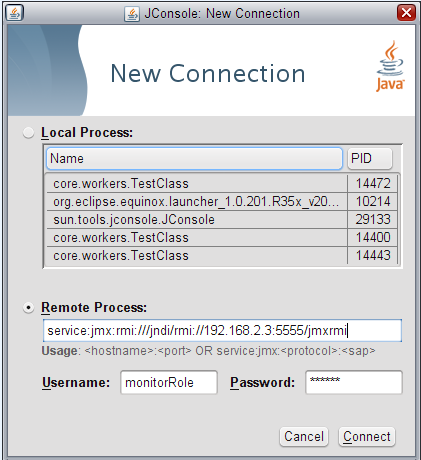
\includegraphics[scale=0.5]{gfx/jconsole.png} 

\subsubsection{Ustawianie �cie�ki przeszukiwa� klas}
Aby mo�liwe by�o dynamiczne �adowanie klas oblicze� konieczne jest wskazanie
scie�ki przeszukiwa� klas (CLASSPATH). Pod t� scie�k� znajduj� si� wszelkie 
achiva JAR, zawieraj�ce poszczeg�lne klasy w kt�rych zawarta jest logika
oblicze�. Tak�e i w tym przypadku konieczna jest modyfikacja skryptu startowego
catalina.sh w kt�rym nale�y doda� nast�puj�cy wpis.
{\tiny
\begin{lstlisting}[style=console, caption=A command] 
CLASSPATH=/opt/tasklibs/*
\end{lstlisting}
}

Aplikacja osadzona na w�z�ach slave zawiera w pliku web.xml cztery parametry
koniguracyjne opisuj�ce gdzie powinna szuka� plik�w bibliotek jak i plik�w
konfiguracji oblicze�.

{\tiny
\begin{lstlisting}[style=console, caption=A command] 
	<context-param> 
    	<param-name>libLocation</param-name> 
    	<param-value>/opt/tasklibs</param-value> 
	</context-param> 

	<context-param> 
    	<param-name>confLocation</param-name>
    	<param-value>/opt/tasklibs/configs</param-value> 
	</context-param> 
	
	<context-param> 
    	<param-name>sshUser</param-name> 
    	<param-value>taskflow</param-value> 
	</context-param> 

	<context-param> 
    	<param-name>sshPassword</param-name>
    	<param-value>taskflow</param-value> 
	</context-param> 
\end{lstlisting}
}

\begin{itemize}
  \item libLocation - zmienna ta pe�ni dwie funkcje. Pierwsz� z nich jest
  dostarczenie informacji sk�d dynamicznie wczytywa� konieczne klasy w momencie
  otrzymania ��dania wykonania jakiego� obliczenia. Drugim zastosowaniem tej
  zmiennej jest dostarczenie informacji serwerowi master do jakiego katalogu
  powinien skopiowa� archiwum JAR pakietu oblicze� na serwerze slave przy u�yciu
  protoko�u SFTP.
  \item confLocation - podobnie jak zmienna libLocation mam za zadanie
  poinformowa� aplikacj� dzia��j�c� na serwerze slave sk�d wczyta� poszczeg�lne
  konfiguracje oblicze�, oraz warto�� tej zmiennej zostanie tak�e u�ytka przy
  wczytywaniu kolejnych plik�w konfiguracji i umieszoczone w odpowiednim
  katalogu na serwerze slave.
  \item sshUser oraz sshPassword - okre�la login i has�o u�ytkwonika na serwerze
  slave kt�ry mo�e zosta� u�yty w celu przetranportowania pliku b�d� konfiguracji b�d� pakietu
  obliczenia za po�rednictwem protoko�u SFTP.
\end{itemize}

Ostatnim elementem konfiguracji aplikacji na serwerach slave jest wpropwadzenie
popwarnych opcji w pliku config.properties (PRZENIESC DO ANT'a).

{\tiny
\begin{lstlisting}[style=console, caption=A command] 
node.jmx.port=5555
node.address=127.0.0.1
node.operation.port=8888
process.server.inetaddr=192.168.2.2
process.server.port=8080
\end{lstlisting}
}

\begin{itemize}
  \item node.jmx.port - okre�la port na kt�ry serwer salve b�dzie m�g� si�
  ��czy� w celu pobrania informacji na temat obecnych parametr�w wirtualnej
  maszyny Javy servera slave.
  \item node.address - okre�la adres IP serwera slave, pole to jest
  konfigurowalne a nie automatycznie wczytywane z uwagi na fakt, �e mo�a sobie
  wyobrazi� slave umieszczony za rozwi�zaniem typu NAT, b�d� dost�p do niego
  mo�e by� realizowany za po�rednictwem tunelu SSH, b�d� innego tego typu
  rozwi�zanie. W takim przypadku adress IP oraz port za po�rednictwem kt�rych
  dost�p jest mo�liwy mog� si� r�ni� od tych ustawie� lokalnych.
  \item node.operation.port - port na kt�rym serwer master b�dzie zleca�
  wykonanie poszczeg�lnych zada� obliczeniowych.
  \item process.server.inetaddr - wskazuje na adres IP serwera master kt�ry
  zostanie u�yty w momencie rejestracji serwera slave.
  \item process.server.port - okre�la port serwera master i po��czeniu ze
  zmienna process.server.interaddr do zarejestrowania si� jakos serwer slave.
\end{itemize}

\subsection{Konfiguracja dziennik�w log4j}
Server glassfish nie posiada wbudowanej obs�ugi systemu dziennikowania log4j.



\chapter{Obliczenia}
\label{cha:obliczenia}
%---------------------------------------------------------------------------

\section{Wprowadzenie}
Aby mo�liwe by�o wykonanie obliczenia na platformie pierwszym krokiem jest
wgranie na serwer pakietu oblicze�, b�d� pliku konfiguracji. Po dokonaniu
walidacji mo�liwe jest utworznie obliczenia, kt�re polega na stworzeniu
bazodanowej reprezentacji obliczenia. Na podstawie tej reprezentacji
silnik realizuje obliczenia zgodnie z konfiguracj� zawart� w pliku
computation.xml zawartego w pakiecie obliczenia, b�d� oddzielnie dodanego pliku
konfiguracji.
\label{sec:wprowadzenie}
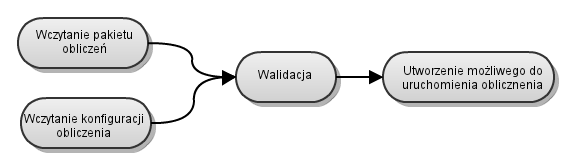
\includegraphics[scale=0.5]{gfx/lifecycle.png}
\newline
Poszczeg�lne elementy oblicze� mog� by� wsp�dzielone pomi�dzy r�ne obliczenia
zale�nie od ich konfiguracji.
W realizacji projektu po�o�ono nacisk na reu�ywalno�c poszceg�lnych sk�adowych
oblicze� a tak�e na �atw� i szybk� konfigurowalno�� ca�ych proces�w oblicze�.
Rozwi�zanie to umo�liwia koponowanie ca�ych proces�w obliczeniowych z mniejszych
sk�adowych.
\newline
Typowa realizacja obliczenia obejmuje nast�puj�ce kroki.
\newline
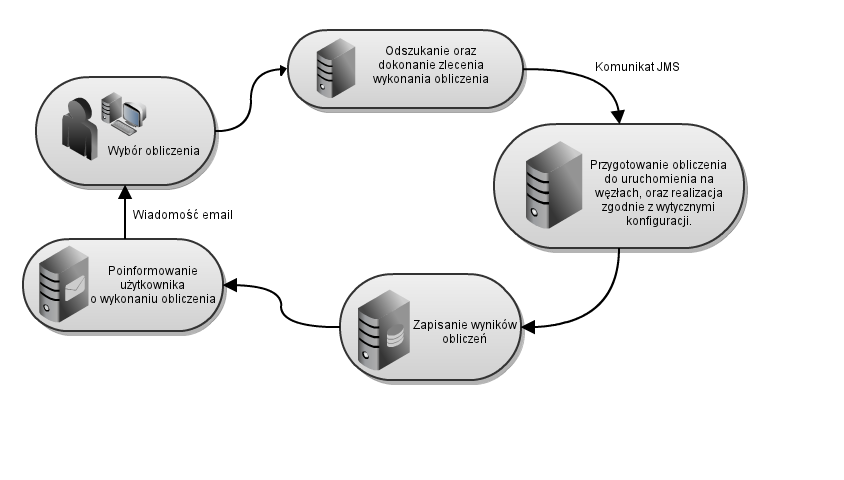
\includegraphics[scale=0.5]{gfx/flow.png}


\section{Pakiety Oblicze�}
\label{sec:pakiety obliczen}
Typowy plik pakietu poblicze� jest typowym archiwum JAR, zawieraj�cym
skompilowane klasy poszczeg�lnych oblicze� wraz z odpowiadaj�cym mu plikiem
konfiguracyjnym opisuj�cym kolejne kroki realizaowanego obliczenia.
\newline
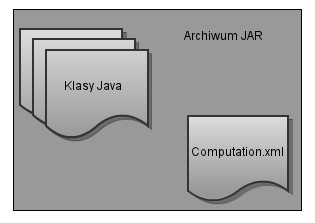
\includegraphics[scale=0.7]{gfx/pakiet.png}
\section{Plik konfiguracji obliczenia}
Elementy pliku konfiguracyjnego.
\begin{itemize}
  \item computation - g��wny element pliku konfiguracyjnego posiadaj�cy atrybut
  Id kt�ry jednoznacznie wyr�nia obliczenie.
  \item description - kr�tki opis ca�ego procesu obliczenia
  \item settings -zawiera list� ustawie� poszczeg�lnych kt�re zostan�
  zastosowane w trakcie realizcacji obliczenia.
  \item setting - pojedyncze ustawienie zawieraj��e atrybut nazwy oraz warto�ci
  jak� ustawienie identyfikowane nazw� otrzyma.
  \item tasks - zawiera list� oblicze� kt�rych dostarcza pakiet oblicze�. Pakiet
  oblicze� mo�e zawiera� wi�ksza liczb� oblicze� nie rzeczywi�cie u�ywa.
  Nadmiarowe definicje oblicze� mog� by� wykorzystywane przez inne konfiguracje
  oblicze�.
  \item task - pojedyncze atomowe obliczenie, z po��czenia wi�kszej ilo�ci
  oblicze� mo�liwe jest tworzenie ca�ych proces�w rezliuj�cych bardziej
  skomplikowane obliczenia. Atrybutami elementu task s� id - jednoznacznie
  wyrozniaj�ce pojedyncze obliczeni, name istotny atrybut, kt�rego warto��
  odpowiada atrybutowi taskName adnotacji @Computable, className - pe�na
  kwalifikowana nazwa klasy zawieraj�ca logike obliczenie globalnie unikalne, 
  konieczne do dynamicznego za�adownia odpowiedniej klasy na
  serwerach slave.
  \item input - stanowi wejscie do pojdeynczego obliczenia zawiera atrybut id
  kt�ry jednoznacznie okre�la wej�cie, name (przypomniec po co?) valueName
  odpowiadaj�cy atrybutowi name adnotacji @Value.
  \item output - stano wyjscie pojdeynczego obliczenia zawiea atrybut name
  (przypomniec po co?) valueName, kt�ry podobnie jak ma to miejsce w przypadku
  wejscia ma warto�� tak� sam� jak atrybut name adnotacji @Value
  \item description mo�e zawiera� opis obliczenia.
  \item transitions Zawiera list� przej�� pomi�dzy poszczeg�lnymi obliczeniami. 
  \item transition opisuje pjedyncze przej�cie pomi�dzy dwoma zadaniami
  obliczeniowymi. Zawiera atrybuty id kt�ry jednoznacznie okre�la globalnie
  pojedyncze przej�cie atrybutr to okre�la wejscie kolejnego zadania
  obliczeniowego, atrybut from definije identygfikator wyjscia poprzeniego
  zadania obliczeniowego.
\end{itemize}

\lstinputlisting[style=source_code, label = some label, caption=A
shellscript,language=Xml]{/home/malczyk/Devel/Java/taskworkflow/ProcessComputationApi/cfg/computation.xsd}

Typowe obliczenie zgodne z powy�szym schematem

\lstinputlisting[style=source_code, label = some label, caption=A
shellscript,language=Xml]{/home/malczyk/Devel/Java/taskworkflow/GeneticCore/cfg/computation.xml}


\section{Silnik Oblicze�-Realizacja obliczenia}
Proces realizacji obliczenia zaczyna si� od zakolejkowania obliczenia.
U�ytkownik uruchamiaj�cy obliczenie powoduje wys�anie komunikatu za
po�rednictwem JMS, kt�ry trafia do kolejki, zawieraj�cy wszystkie konieczne
startowe parametry takie jak ustawienia obliczenia oraz warto�ci startowe 
pierwszego z oblicze� w procesie. Po otrzymaniu komunikatu o uruchomieniu
obliczenia nast�puje jego realizacja. 
Pierwszym krokiem jest ustawienie warto�ci
pocz�tkowych parametr�w. Kolejnym krokiem jest wczytanie definicji procesu
obliczenia z bazy danych, oraz utworzenie odpowiedniej wygodnej do u�ycia
reprezentacji procesu obliczenia. W dalszej cz�ci silnik oblicze� przesuwa si�
po grafie zgodnie z zdeginiowanymi przej�ciami wykonuj�c kolejne obliczenia.
Silnik oblicze� w momencie realizacji precesu zarz�dza swoj� przestrzenia
zmiennych zawieraj�ce nazwy oraz odpowiednie warto�ci, kt�re mog� by�
uaktualniane. Po realizacji pojedynczego obliczenia warto�� jego wyj�cia 
tj. warto�� sk�adowje obiektu oznaczonej adnotacja @Value oraz atrybutem
valueName wyjscia jest przechowywana i mo�e pos�u�y� jako wej�cie dowolnego
kolejnego zadania obliczeniowego. Wykonanie pojedynczego zadania obliczeniowego
rozpoczyna si� od ustalenia na podstawie odpowiednich informacji zawartych w
konfiguracji obliczenia kt�re zadanie jest kolejnym kt�re powinno by�
realizowane. 
Po ustaleniu tej informacji kolejnym krokiem b�dzie ustawienie
warto�ci na wej�cia zadania obliczeniowego. W dalszej cz�sci dobierany pozostaje
w�ze� obliczeniowy slave, kt�ry zrealizuje obliczenie. Tu� po okre�leniu
kt�ry w�ze� zosta� wybrany, dokonywana jest serializacja warto�ci wejsci� oraz
wys�anie przy pomocy protoko�u HTTP wraz z Hessian rz�dania wykonania
obliczenia. Serwer slave po trzymaniu rz�dania okre�la kt�re zadanie
obliczeniowe powienien wykona� na podstawie atrybutu taskName. Kolejnym
poczynionym przez niego krokiem jest sprawdzenie w swojej pami�ci podr�cznej czy
dla zadnego zadania obliczenia istnieje za��dowan ju� klasa obiektu realizuj�ca
obliczenie. W przypadku braku takiej informacji aplikacja na serwerach slave
przeszukuje wszystkie archiva JAR, kt�re znajdzie na swojej �cie�ce przeszukiwa�
w celu znalezienia odpowiedniej klasy. Gdy kalsa zosta�a znaleziona przy pomocy
mechanizm�w reflesksji j�zyka Java tworzony jest obiekt obliczenia, oraz
ustawiane s� warto�ci na jego wej�ciach. W dalszej cz�sci wykonywane jest
w�a�ciwe obliczenie. Po dokonaniu odpowiednich oblicze� warto�ci zmiennych kt�re
pos�u�� jak wyj�cia zostan� ustawione z odpowiednimi warto�ciami. Warto�ci z
wyj�� zosta� za po�rednictwem narz�dzia XStream zserwalizowane oraz zr�cone do
serwera Master. Serwer master po otrzymaniu wynik�w z serwera slave zapisze je
do swojej pami�ci w celu dalszego wykorzystania. Te czynno�ci wykonywane b�d�
tak d�ugo jak d�ugo pozostan� pojedyczne sk�adowe obliczenia do wykonania.
Po dokonaniu wszystkich oblicze� warto�ci wszystki wyj�c, z kr�rego kolowiek
zadania obliczeniowego oznaczonych jako result zostan� zapisane w bazie i b�d�
stanowi�y ostateczny wynik obliczenia. Po zako�czeniu obliczenia, b�d� w
przypadku b��du w trakcie jego realizacji u�ytkownik kt�ry zainicjowa� wykonanie
obliczenia zostanie poinformowany za po�rednictwem wiadomo�ci elektronicznej
email o sukcesie wraz z adresem URL do strony sk�d b�dzie m�g� sci�gn�c wyniki
oblicze� b�d� te� b��dzie obliczenia. I tym przypadku rz�dzanie o wys�anie
wiadomo�ci email odbywa si� w spos�b asynchroniczny za pomoc� JMS.

\section{Uruchamianie obliczenia}

\section{Prezentacja Wynik�w}
Wyniki oblicze� przechowywane s� w formacie XML. Zawieraj� one dane jawnie
wyspecyfikowane w konfiguracji obliczenia. Spos�b prezentacji oblicze� jest
wpe�ni konfigurowalny.
\newline
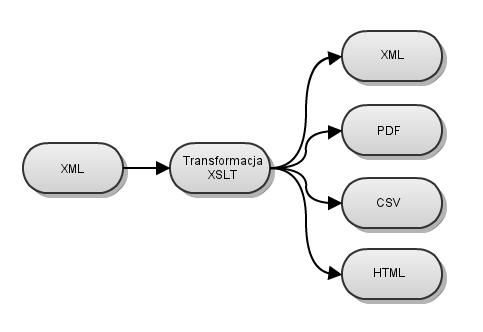
\includegraphics[scale=0.5]{gfx/present.png}
\newline
Dodanie kolejnych metod prezentacji wynik�w oblicze� wymaga stworzenia i dodania
do systemu pliku transformaty XSL. W momencie pr�by pobrania na liscie 
rozwijalej pojawi si� mo�liwo�� wybrania transformaty, kt�ra na�o�ona zostanie
na plik XML wyniku a nast�pnie wynikikowy plik b�dzie mo�liwy do �ci�gni�cia.

\section{Interfejs Programownia (API)}

\subsection{Przyk�adowe obliczenie}
Poni�szy przyk�ad ukazuje implemetacj� prostego pojedynczego zadania
obliczeniowego, kt�re mo�e by� w��czone w ca�y proces. Zadanie obliczeniowe
dokonuje ewaluacji poszczeg�lnych osobnik�w populacji poprzez wyliczenie
warto�ci funkcji DeJonga. 
\newline

\[F(x_{1}, x_{2}, \ldots, x_{i}) = \sum_{i=1}^{n} x_{i}^{2}\]

Pojedyncze zadanie obliczeniowe mo�e by� postrzegane nast�puj�co.
\\
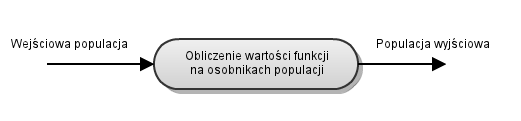
\includegraphics[scale=0.8]{gfx/task.png}
\\

\lstinputlisting[style=source_code, label = some label, caption=A shellscript,language=Java]{/home/malczyk/Devel/Java/taskworkflow/GeneticCore/src/genetic/tasks/DeJongEvaluator.java} 

Opisac\ldots



\subsubsection{Adontacje j�zyka Java}
Tworzenie oblicze� na platform� polega na dostarczeniu obiekt�w enkapsuluj�cych
logik� obliczenia, kt�re b�d� implementowa�y odpowiednie interfejsy oraz b�d�
odpowiednio zaadnotowane. Dost�pne adnotacje Javy to
\begin{itemize}
  \item Computable - Klasy zaadnotowane adnotacja @Computable b�d�
  rozpoznane jako mo�liwe do uruchomienia na platformie. Adnotacja ta posiada
  atrybut taskName na podstawie kt�rego sewer slave odnajduje odpowienia klas�
  obliczenia tworzy jego instancj� i wywo�uje metod� doComputation()
  zdefiniowan� w interfejsie ComputableTask, kt�ry ka�de zadanie obliczeniowe
  musi implementowa�.
  \item Routable - Dotyczy klas zada� obliczeniowy kt�re dodatkowo maj�
  mo�liwo�� sterowania przebiegiem obliczenia (zap�tle�, rozga��zie�), zale�nie
  od pewnych czynnik�w.
  \item RouteTo - Stosowane wraz z adnotacj� @Routable okre�la kolejne wej�cie
  nast�pnego zadania.
  \item ComputationContext - Pola klasy oznaczone t� adnotacj� b�d� mia�y obiekt
  przechowuj�cy informacj� o ustawieniach obliczenia oraz bie��cym statnie tego�
  obliczenia.
  \item Value - Sk�adowe klasy zaadnotowane t� klasa przechowuj� warto�ci, kt�re
  mog� pos�u�y� jako wej�cia obliczenia, b�d� jako jego wyj�cia tj. Obliczenia.
  \item Partitionable - Obliczenia wykonanywane na warto�ciach sk�adowych klas
  oznaczonych adnotacj� @Partitionable mog� zosta� podzielone i wykonywane
  r�wnolegle na wielu kolekcjach. Przyk�adem tutaj mo�e by� obliczenia funkcji
  przystowowania populacji osobnik�w. Gdzie wej�ciem obliczenia jest ca�a
  populacja, kt�ra dzielona jest na r�nej wielko�ci fragmenty, zale�nie od
  ilo�ci aktualnie dost�pnych serwer�w slave. Po wykonaniu obliczenia wyniki
  s� ��czone i przypisywane do odpowiedniego wyj�cia.
\end{itemize}

\subsection{Tworzenie procesu obliczenia}

\label{sec:api}




\bibliography{bibliografia}

\end{document}
